\icode{E-O-CA-L3-261003-001}
光纤通讯已成为现代主要的有线通讯方式。现有一长为\qty{1}{km}，直径为\(d =\) \,\qty{0.2}{mm}的长直光纤，一束单色平行光从该光纤一端沿光纤方向射入，延时\qty{5e-6}{s}在光纤另一端接收到时该光束。求：
\begin{enumerate}
	\item 光纤的折射率；
	\item 如图所示该光纤绕圆柱转弯，若平行射入该光纤的光在转弯处均能发生全反射，求该圆柱体半径\(R\)的最小值。
\end{enumerate}

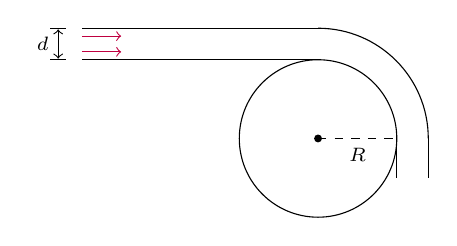
\begin{tikzpicture}[font=\scriptsize]
	\draw (0,1)--(-3,1) (0,1.4)--(-3,1.4) (1,0)--(1,-.5) (1.4,0)--(1.4,-.5);
	\draw (0,0) circle(1);
	\fill (0,0) circle(.05);
	\draw (1.4,0) arc(0:90:1.4);
	\draw[|<->|] (-3.3,1.4)--node[left]{\(d\)}(-3.3,1);
	\draw[dashed] (0,0)--node[below]{\(R\)}(1,0);
	\draw[->,purple] (-3,1.1)--(-2.5,1.1);
	\draw[->,purple] (-3,1.3)--(-2.5,1.3);
\end{tikzpicture}
\begin{answer}
    （1）\(n = 1.5\)（2）\(R_{\min} =\) \qty{0.4}{mm}\qquad 提示：分析可知，如下图所画光线对应的入射角最小，光应在这发生全反射

    \begin{tikzpicture}[decoration={markings,mark=at position 0.5 with {\arrow{>}}},font=\scriptsize]
	\draw (0,1)--(-3,1) (0,1.4)--(-3,1.4) (1,0)--(1,-.5) (1.4,0)--(1.4,-.5);
	\draw (0,0) circle(1);
	\fill (0,0) circle(.05);
	\draw (1.4,0) arc(0:90:1.4);
	\draw[|<->|] (-3.3,1.4)--node[left]{\(d\)}(-3.3,1);
	\draw[dashed] (0,0)--node[below]{\(R\)}(1,0);
	\draw[->,purple] (-3,1.1)--(-2.5,1.1);
	\draw[->,purple] (-3,1.3)--(-2.5,1.3);
    \draw[postaction={decorate},purple] (0,1)--({.4*sqrt(6)},1)coordinate(c);
    \draw[dashed,cyan] (0,0)--(c) (0,0)--(0,1);
    \end{tikzpicture}
\end{answer}